In diesem Teil werden alle theoretischen Informationen gegeben, die man für das Verständniss des ganzen Projektes braucht. Nach dieser Einführung sollte man in der Lage sein, den Quellcode im Anhang zu verstehen. Da es jedoch sehr viel Übung erfordert, einen Quellcode zu lesen und zu verstehen, ist es naheliegend, dass der Quellcode nicht verstanden wird. In der Einführung wird grob angeschaut, wie man überhaupt vom Quellcode zur App kommt, im zweiten Teil wird erklährt, wie Daten jeglicher Art als Zahlen in einem Computer abgespeichert werden, im dritten Teil gibt es eine Einführung in die Programmiersprache Java und im letzten Teil werden dann noch ein paar spezifische Informationen in bezug auf Java gegeben, die für die Erstellung einer App gebraucht werden und die Software "`Android Studio"' wird erklährt.

\subsection{Einführung}
\subsubsection{Die IDE}
Die IDE (eng. integrated development environment) oder auf Deutsch die Entwicklungsumgebung ist der Ort, an dem die meisten Programmierer arbeiten. Sie bietet alle wichtigen Werkzeuge, die man zum entwickeln von Software benötigt (Editor mit Color Highlighting, Compiler, Debugger, Dateibrowser etc.). Auf einige Begriffe wird später noch genauer eingegangen. In unserem Falle heisst die Entwicklungsumgebung übrigens Android Studio. In der Entwicklungsumgebung findet die ganze Entwicklung einer Software statt. Der wichtigste Bereich davon ist der Editor. Dort wird der ganze Quellcode hingeschriben und dank Color Highlighting werden die wichtigen Komponenten (Kontrollstrukturen, Variablen, Kommentare etc. siehe Abschnitt 2.3 Grundlagen von Java) mit Farbe hervorgehoben (Abbildung \ref{fig:Colorhighlighting}).
\begin{figure}[htbp] 
  \centering
     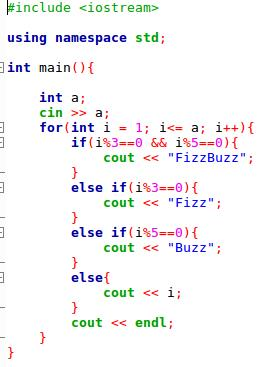
\includegraphics[width=0.3\textwidth]{CodeColor.jpg}
     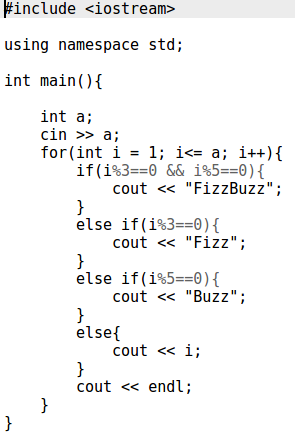
\includegraphics[width=0.3\textwidth]{CodeWithoutColor.png}
  \caption{Beispiel mit und ohne Farbhervorhebung \cite{Colorhighlighting}}
  \label{fig:Colorhighlighting}
\end{figure}
Das ist sehr wichtig, da man ansonsten schnell den Überblick verloren hat. Natürlich gibt es nicht nur eine IDE sondern ganz viele. Welche man davon benutzt ist jedem selbst überlassen. Es gibt auch Entwickler, die es bevorzugen, ohne eine IDE zu arbeiten. Zwar kann man dann alles selbst so gestallten wie es einem passt, es macht aber alles viel komplizierter ist besonders für neu beginnende Programmierer nicht empfehlenswert.

\subsubsection{Der Compiler}
Leider versteht der Computer nichts von dem, was wir in den Quellcode schreiben, alles was er versteht besteht aus Nullen und Einsen (mehr darüber im Abschnitt 2.2). Deshalb muss der für uns verständliche Quellcode in Maschinencode übersetzt werden. Dies geschieht mit dem so gennanten "`Compiler"' (eng. to compile = zusammentragen). Meistens ist dieser bereits in der IDE enthalten und auf Knopfdruck abrufbar. 

\subsubsection{Der Debugger}
Der Debugger ist sehr eng mit dem Compiler verbunden. Meistens schafft man es nähmlich nicht, auf Anhieb einen Fehlerlosen Code zu schreiben. Es passiert extrem schnell, dass irgendwo ein "`;"' oder eine Kontrollstruktur falsch geschrieben wurde (mehr dazu im Abschnitt 2.3). Deshalb ist es sehr wichtig, dass man den Fehler findet. Wenn man jetzt aber Quellcode von 500 Zeilen geschrieben hat, wäre es doch sehr mühsam, wenn man nur wüsste, dass man einen Fehler hat. Genau dafür ist der Debugger. Ist aus dem englischen Wort "`Bug"' entstanden, was so viel wie Käfer heisst, im Programmieren aber als Synonym zu Fehler verwendet wird. Dementprechend könnte man also Debugger als "`Entfehlerer"' oder verdeutscht als "`Fehlersuchprogramm"' bezeichnen. Meistens wird er aber einfach Debugger gennant. Offenbar ist der Debugger dazu in der Lage, die Programmierfehler zu finden. Er findet aber leider nur Syntaxfehler und keine, die den gewünschten Programmoutput betreffen. Man kann sich das so vorstellen: In Microsoft Word werden auch Rechtschreibefehler angezeigt, trotzdem kann man Sätze bilden die entweder keinen Sinn ergeben oder etwas anderes Aussagen, als gewünscht. Aber der Programmieraltag ohne Debugger wäre fast unvorstellbar, da man die meisten Fehler nicht so einfach sieht wie ein falsch geschriebenes Wort. Es gibt verschiedene Arten von Debugger. Die meisten zeigen einem die Fehler erst an, wenn man den Quellcode zu komplieren versucht, es gibt aber auch solche, die das in Echtzeit machen, so wie Microsoft Word Rechtschreibefehler anzeigt. 

\subsubsection{Die Programmiersprache}
Eine Programmiersprache kann man sich am einfachsten wie eine richtige Sprache vorstellen. Sie bildet den Grundbaustein des Programmierens. Bevor man dem Computer etwas  beibringen kann, muss man eine solche lernen. Jede Programmiersprache hat seine eigene Syntax, trotzdem sind sie meistens ähnlich aufgebaut. Sobald man also eine Programmiersprache gelernt hat, fällt es einem einfach, eine nächste zu lernen. Man muss sich das so vorstellen: Nachdem man gelernt hat, wie Windows XP funktioniert, hat man nicht mehr so grosse Schwierigkeiten, zu lernen wie Windows 7 oder Windows 8 funktioniert. Meistens haben die Programmiersprachen verschiedene Anwendungsbereiche: Wird z. B. JavaScript und PHP meist nur in Webanwendungen verwendet, wird C++ wegen seiner Geschwindigkeit meist in Systemanwendungen gebraucht oder Java für Geräte wie Drucker oder eben Androidapplikationen, ausserdem ist das berühmte Computerspiel "`Minecraft"' in Java geschrieben.
\subsection{Vom Binärcode zum Bild}
In diesem Teil geht es darum zu verstehen, wie ein Computer komplexe Informationen wie Bilder speichern kann. Dazu geht man zuerst von Binärcode (z.B. 01110110101001) aus und arbeitet sich dann hoch. Zwar ist dieses Thema nicht unbedingt notwendig, um unser Projekt nachvollziehen zu können, aber es hilft dabei, sich die Datenspeicherung besser vorstellen zu können, was auf jeden Fall sinnvoll ist, da ja die Datenspeicherung eines unserer Kernthemen ist. Ausserdem kann man dann auch die Datentypen in Java besser verstehen (Abschnitt 2.3).
\subsubsection{Vom Binärcode zur Zahl}
Die kleinste Speichereinheit eines Computers ist das Bit. Man sollte das Bit aber auf keinen Fall mit dem Byte verwechseln. Das Byte beinhalted nämlich acht Bits und ist dadurch viel grösser als das Bit. Man kann sich das Bit als Schalter vorstellen: Entweder ist er an oder er ist aus. Es gibt genau diese 2 Zustände. Mit der 1 bezeichnet man den angeschalteten Zustand und mit 0 den ausgeschalteten. Wenn man jetzt zwei Schalter nimmt dann gibt es bereits 4 verschiedene Schalterzustände: 00, 01, 10 und 11. Wenn wir nun $N$ Schalter anneinander reihen haben wir dementsprechend dann auch $2^N$ verschiedene Schalterzustände. Wenn wir jetzt jeden dieser Schalterzustände einer Zahl zuordnen, kann man je nach Schalteranzahl beliebig grosse Zahlen abspeichern. Jedoch wurden Zahlen nicht willkürich irgendeiner Schalterkombination zugeordnet sondern es gibt ein gewisses System dahinter, damit man die Zahlen nachher auch miteinander verrechnet werden können. Dieses System nenn man das binäre Zahlensystem. Es ist nicht wie unser dezimales Zahlensystem auf zehn ausgerichted sondern auf zwei. Um die Zahlen schreiben können, muss aber zuerst deffiniert werden, wie viele Bits gross eine Zahl ist. Diese Definition wird hier der Einfachheit halber auf 4 Bits gesetzt. Wie auch in unserem Zahlensystem wird die Zahl 0 als 0 dargestellt. Weil aber 4 Bits zur Verfügung stehen und nicht nur eines, müssen wir auch den anderen 3 einen Zustand geben, also auch 0. Dann sieh die Zahl 0 also binär dargestellt so aus: 0000. Auch die Zahl 1 ist noch eifach darzustellen: 0001. Wenn aber die Zahl 2 geschrieben werden soll, wird es bisschen komplizierter. Wir können nämlich den ersten Schalter nicht auf auf 2 Stellen. Die Antwort ist aber eigentlich ganz einfach: Wie in unserem dezimalen Zahlensystem nach der Zahl 9 eine neue Stelle gebraucht wird, so wird es binär genau gleich nach der Zahl 1 gemacht. Deshalb wird die Zahl 2 also so geschrieben: 0010. In diesem System geht es weiter: \\
\\
\begin{tabular}{l|l|l|l|l|l|l|l|l|l|l}
Dezimal & 0 & 1 & 2 & 3 & 4 & 5 & 6 & 7 & 8 &  ...\\ \hline
Binär & 0000 & 0001 & 0010 & 0011 & 0100 & 0101 & 0110 & 0111 & 1000 & ...\\
\end{tabular}  \\
\\
Dieses System gut zu kennen kann sehr nützlich sein. Wenn man die Zahlen nämlich noch ein bischen genauer analyziert, kann man feststellen, dass man die hinterste Stelle der binären Zahl immer angibt, ob der Zahl eine 1 addiert werden muss, die zweit hinterste dasselbe mit 2, der dritt hintersten mit 4. Bei jeder weiteren Stelle nach vorne nimmt die dazuzuaddierende Zahl um den Faktor 2 zu. Wenn man dieses System erkannt hat, kann man auch grosse binäre Zahlen in einer nützlichen Frist in eine dezimale übersetzten und umgekehrt. Hier ein Beispiel mit der achtstelligen Binärzahl 10100101:
\\
\begin{tabular}{l l l l l l l l l l l l l l l l l}
$1$ & & $0$ & &  $1$ & & $0$ & & $0$ & & $1$ & & $0$ & & $1$ & & \\
$ 128 $ &+& $0$ &+& $ 32$ &+& $0$ &+& $0$ &+& $ 4$ &+& $0$ &+& $1$ &=& $165$ \\ 
\end{tabular} \\
\\
Das hier vorgestellte binäre Zahlensystem ist jedoch stark vereinfacht, da sich in diesem nur Zahlen $\in \mathbb{N} $ darstellen lassen. Negative Zahlen und Gleitkommazahlen würden aber zu stark vom eigentlichen Thema abweichen. Wichtig ist nur, dass der Computer nur so gennante Maschienenzahlen abspeichern kann. Das heist die Zahlen müssen endlich gross sein und deshalb können periodische und irrationale Zahlen nicht genau abgespeichert werden.
\subsubsection{Grundoperatoren bei binären Zahlen}
Wenn man erst mal verstanden hat, wie das binäre Zahlensystem funktioniert, dann sind die Grundoperationen sehr einfach. Sie lassen ganz einfach mit den schriftlichen Operationen berechnen. Als Beispiel werden 5 Bit grosse Zahlen genommen: Die Zahl 6 (00110) und die Zahl 3(00011).
\paragraph{Addition}
\begin{tabular}{llllll}
&0&0&1&1&0 \\
+&0&0&0&1&1 \\ \hline
&0&1&0&0&1
\end{tabular}
\paragraph{Subtraktion}
\begin{tabular}{llllll}
&0&0&1&1&0 \\
-&0&0&0&1&1 \\ \hline
&0&0&0&1&1
\end{tabular}
\paragraph{Multiplikation}
\begin{tabular}{lllllllllll}
0&0&1&1&0& $\cdot$ &0&0&0&1&1 \\ \hline
&&&&&&0&1&1&0&0 \\
&&&&&&0&0&1&1&0 \\ \hline
&&&&&&1&0&0&1&0
\end{tabular}
\paragraph{Division}
\begin{tabular}{lllllllllll l}
0&0&1&1&0& : &0&0&0&1&1 & = 0 0 0 1 0 \\ \hline
 & &1&1& & &&&&&& \\ \cline{3-4}
 & &0&0&0& &&&&&& \\ 
\end{tabular}
\subsubsection{Von der Zahl zur Text}
Mit dem Wissen, wie Zahlen binär gespeichert werden, kann man dann sehr eifach verstehen, wie Texte abgespeichert werden. Im Grundsatz ist es nur eine willkürliche Zuordnung von Zeichen zu einer Zahl. Es gibt verschiedene Zuordnungen, die wichtigsten hierbei sind ASCII (American Standart Code for Information Interchange) und UTF-8(Universal Character Set Transformation Format). ASCII hierbei speichert jegliche Zeichen in 7 Bits ab und kann aber nur 128 verschiedene Zeichen speichern. Zum Beispiel würde man das Wort Haus so kodieren: 72 97 117 115. Wenn man diese Zahlen auch noch in Bits übersetzt, hat man die exakte Kodierung, wie sie auch auf dem Computer abgespeichert würde: 1001000110000111101011110011(siehe Abbildung \ref{fig:ASCII})
\begin{figure}[htbp] 
  \centering
     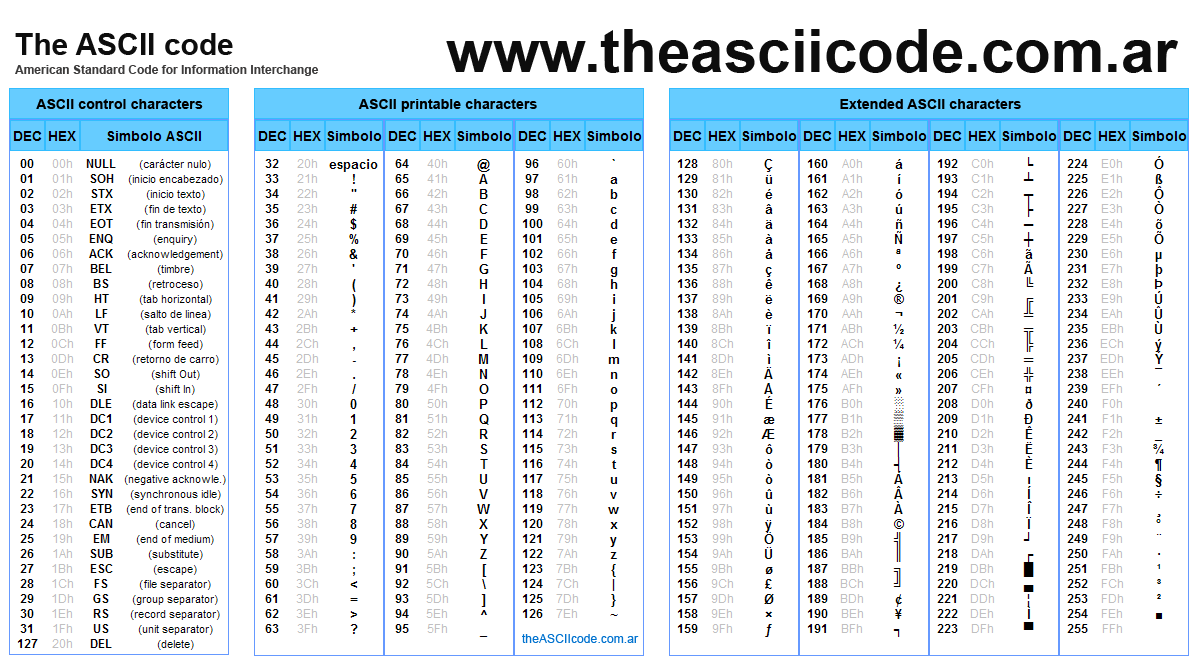
\includegraphics[width=1\textwidth]{ASCII.png}
  \caption{ASCII Tabelle \cite{ASCII}}
  \label{fig:ASCII}
\end{figure}
Dadruch werden viele sprachspezifischen Zeichen wie die deutschen Umlaute nicht abspeicherbar. Deshalb wird ASCII heutzutage auch meistens nicht mehr gebraucht. UTF-8 ist hierbei viel nützlicher, aber auch komplizierter. Es kann jegliche Spezialzeichen jeder Sprache abspeichern. UTF speichert die einfachen ASCII Zeichen in 8 Bits ab, das erst hinzugekommene Bit speichert ab, ob es sich bei dem Zeichen um ein ASCII Zeichen handelt oder nicht. Falls ja, können die restlichen sieben Bits wie ein ASCII Zeichen interpretiert werden. Ansonsten folgen nicht nur 7 Bits sondern wieder abhängig von der nächsten Zeichenfolge bis zu 31 weitere Bits (im ganzen dann 4 Bytes). Die deutschen Umlaute brauchen zum Beispiel 2 Bytes Speicherplatz. UTF-8 ist heutzutage der meist verbreitete Zeichensatz im Internet (im November 2016 benutzen rund 88\% aller Webseiten UTF-8). \cite{UTF-8} Ein weiterer heutezutage sehr verbreiteter Zeichensatz ist Unicode, auf diesen wird hier aber nicht weiter eingegangen.
\subsubsection{Von der Zahl zur Farbe}
Um Bilder abspeichern zu können, muss man zuerst einmal wissen, wie Farben abgespeichert werden. Die meist verbreitete Methode für das Abspeichern von Farben ist RGB (eng. Red Green Blue). Der Name spricht für sich, nacheinander wird die Menge der Farbe Rot, Grün und Blau in einer Skala von 0 bis 255 angegeben. Aber auch die Farben werden in einem unüblichen Zahlensystem dargestellt: im Hexadezimalen. Dieses basiert nicht wie das binäre auf 2 und das dezimale auf 10, sondern auf 16. Da in unserem Zahlensystem keine Ziffer für 10-15 existieren, hat man dier ersten Buchstaben des Alphabetes genommen. 10 wäre also "`A"' und 15 wäre "`F"' hexadezimal geschrieben. \textbf{Achtung: Wegen diesem System ist die hexadezimale 10 nicht dasselbe wir die dezimale 10 sondern 16.} 255 wäre dementsprechend "`FF"' hexadezimal geschrieben und somit die grösste hexadezimale Zahl, die mit zwei Ziffern geschrieben werden kann. Das ist natürlich kein Zufall sondern extra so gewählt. Um eine hexadezimale Zahl zu kennzeichnen, benutzt man in der Regel den Präfix 0x. Ein RGB wert besteht also aus drei zwei stelligen hexadezimalen Zahlen. Meistens wird bei RGB-Farben ein \# als Präfix verwendet anstatt des hexadezimal üblichen 0x. Auch noch wichtig anzumerken ist, dass das RGB-System ein additiver Farbraum ist. Das heisst also wenn man die volle Farbstärke aller Farben Rot, Grün und Blau verwendet, erhält man weiss. Hier nun eine Tabelle mit den wichtigsten Farben und dem dazugehörigen hexadezimalen Wert. \\
\\
\begin{tabular}{|l|l|l|l|}
\hline
Rot & Grün & Blau & Weiss \\ \hline
\#FF0000  & \#00FF00 & \#0000FF & \#FFFFFF \\ \hline\lstset{language=Pascal} 
Schwarz & Gelb & Magenta & Cyan \\ \hline
\#000000 & \#FFFF00 & \#FF00FF & \#00FFFF \\ \hline
\end{tabular} \\
\\
Übrigens ist es auch kein Zufall, dass die Farben hexadezimal dargestellt werden und nicht dezimal. Ein System, welches auf zehn basieren würde, hätte immer ein gewissen Datenverlust, da man um 10 darstellen zu können 4 Bits braucht. Mit 4 Bits lassen sich aber Zahlen bis 16 darstellen. Um also mit demselben Speicherbedarf die maximale Speicherausnutzung zu erreichen, hat man sich für ein hexadezimales System entschieden. Es gibt auch hier nicht nur ein System, ein weiteres sehr wichtiges Farbsystem ist das "`CMYK"', welches vor allem für Drücker verwendet wird. Dieses System ist im Gegensatz zum RGB-Farbsystem ein subtraktives. Der Name steht für Cyan Magenta Yellow Key. Auch wie im RGB-Farbsystem werden mit Cyan, Magenta und Gelb die Menge der Farben dargestellt. Das CMYK-Farbsystem besitzt aber noch einen vierten Wert: Den Schwarzanteil (hier mit K für Key angegeben um nicht mit B für Black um eine Verwechslungsgefahr mit Blue zu vermeiden).
\subsubsection{Von der Farbe zum Bild}
Nun sollten alle Grundlagen vorhanden sein, um zu verstehen, wie ein Bild gespeichert werden kann. Hier wird zuerst von einem total unkomprimierten Bild ausgegange, das mit RGB Farben ausgestattet ist. Digitale Bilder können in zwei Gruppen unterteilt werden: Rastergrafiken und Vektorgrafiken. Zuerst wir ersteres angeschaut. Ein Computerbildschirm ist bekanntlicherweise aus einzelnen Pixeln aufgebaut. Jedes dieser Pixel funktioniert eigenstädnig und kann eine belibige Farbe anzeigen. Heutzutage ist das wohl am weitesten Verbreitete Bildschirmformat das Full-HD mit 1920x1080 Pixeln. In einem völlig unkomprimierten Bild wird also für jedes Bild seine eigene Farbe gespeichert und schon hat man sein Bild abgespeichert. Wir aber aus dem letzt Kapitel über Farben bekannt ist, werden die Farben üblicherweise mit RGB abgespeichert. Wenn man nun bedenkt, wie diese Zahlen binär aufgebaut werden, kommt man für jede hexadezimale Stelle auf 4 Bits, die gebraucht werden. Weil eine normale RGB-Farbe aus 6 hexadezimalen Zahlen bestehen, heisst das wiederum, dass eine RGB-Farbe mit 24 Bits geschriben werden kann, was das gleiche wie 3 Bytes ist. Um also ein Bild abzuspeichern, werden $1920 \cot 1080 \cdot 3=6220800$ Bytes $ \approx  6.5$ Megabytes. Das ist bereits eine sehr grosse Datenmenge. Für Qualitativ hochwertige Bilder ist die Auflösung aber oftmals grösser und die Farbe genauer, wodurch der Bildspeicherplatzbedarf nochmals enorm wachsen würde. Wenn man jetzt sogar ein Video mit 60 FPS (eng. Frames Per Second = Bilder pro Sekunde) mit dieser Datengrösse des errechnetetn Bildes mit 6.5MB  speichern würde, würde man für jede Sekunde 390MB verbrauchen. Dadurch wäre also ein Film mit einer durschnittlichen Länge von 1.5h 2.106TB gross, also grösser als die meisten Speicher eines Computers. Die Realität sieht aber ganz anders aus: Um Speicherplatz zu optimieren werden erstens bei Bildern komprimierungen angewendet, welche über komplexe Algorithmen die Bilder so abspeichern, dass diese viel weniger Speicherplatz einnehmen. Ausserdem speichern Videos nicht jedes Bild neu sondern nur dessen Veränderung. So kommt man dann auf eine etwa 1000 mal kleinere Speichergrösse. Bei Bildkompression unterscheidet man übrigens auch zwischen verlustbehafteten Kompressionen und verlustfreien. Bekannte verlustfreie Kompressionen sind zum Beispiel TIFF und PNG und bekannte verlustbehaftete JPEG und GIF \cite{Dateiformate}. Jedes Dateiformat hat aber seine eigenen Vorteile und Nachteile und je nach Zweck solle man sich überlegen, welches davon am meisten Sinn macht. Wie Anfangs erwähnt gibt es aber auch noch die Vektorgrafik. Die Vektorgrafik speichert keine Informationen über einzelne Pixel sondern es speichert zum Beispiel eine Linie oder ein Kreis mit einer Funktion. Der Vorteil einer Vektorgrafik ist, dass man diese frei skalieren kann, ohne dass man eine Qualitätseinbusse hat. Meistens sind Firmenlogos und Ähnliches mit einer Vektorgrafik gezeichnet.
\subsection{Grundlagen von Java}
Jetzt da alles nötige erarbeitet wurde, um sich auch etwa vorstellen zu können, wie ein Computer Informationen speicheren kann, wird es einfach werden, die Datentypen von einer Programmiersprache wie Java zu verstehen. Im Abschnitt "`Grundlagen von Java"' wird die Programmiersprache schnell überflogen, so dass jemand, der bereits eine andere Programmiersprache kennt, Java schnell begreifen sollte und den Code im Anhang verstehen können sollte. Da jedoch keine praktischen Aufgaben gestellt werden und auch nicht alles im Detail angeschaut wird, sind diese Grundlagen nicht dazu geignet, nach diesen selber entwickeln zu können. Für jene, die noch über keine Grundlagen über eine Programmiersprache verfügen, könnte dieser Einstieg zu schwierig sein und auch für jene, die über eine umfassende und vertiefte Erklährung wünschen, empfehlen wir eine andere Wissensquelle. Die Fachhochschule Südwestfahlen hat zum Beiepiel ein schönes Skript zur Einführung in Java geschriben \textbf{https://www4.fh-swf.de/media/java.pdf}. Wer lieber ein Buch zur Hand nimmt, dem können wir O'Reilly's "`Java von Kopf bis Fuss"' oder 	"`Java ist auch eine Insel"' empfehlen, die ein solides Grundwissen vermitteln.
\subsubsection{Die Main-Methode}
In Java liegt der Einstiegspunkt in das Programm immer in der Main-Methode. Diese Klasse wiederum liegt in einem Package und das Package im Projektordner. Fürs erste steht aber nur die Klasse im Fokus. Die Packages dienen hierbei einzig und allein der Struktur, wie Ordner auf dem Betriebssystem. Sobald der Compiler die Main-Methode endeckt (unten aufgeführt) erkennt er diese als Einstiegspunkt an. Im Normalfall wird auch die Klasse "`main"' gennant, um den Ort der Main Methode sofort ersichtlich zu machen. In eben dieser Main Methode können jetzt beliebige Befehle geschrieben werden. Im Code unten wird zum Beispiel eine Konsolenausgabe gemacht, der Wohl wichtigste Befehl. Innerhalb der Anführungs- und Schlusszeichen kann ein beliebiger Text geschrieben werden, der dann vom Programm in der Konsole ausgegeben wird.
\begin{lstlisting}
public class main { //erstellt eine neue Klasse mit dem Namen main
	public static void main(String[] args) { //Beginn der Main Methode
		System.out.println("Hello World!"); //erzeugt eine Konsolenausgabe mit dem Text Hello World
	}	//Ende der Main Methode
}
\end{lstlisting}
Konsole:
\begin{lstlisting}[style=console]
Hello World!
\end{lstlisting}
\subsubsection{Datentypen}
\paragraph{Einfache Datentypen}
Im Kapitel 2.2 "`Vom Binärcode zum Bild"' wurde bereits ausführlich beschrieben, wie ein Computer die Daten abspeichert. Um einer Programmiersprache zu sagen, dass sie etwas abspeichern soll, muss man eine Variable definiert werden. Es gibt hierbei verschiedene Variabeln, die unterschiedlich gross sind und auch unterschiedliche Variablen abspeichern können.
\begin{lstlisting}
public class main {
	public static void main(String[] args) {
		boolean b; //Speichert einen Wahrheitswert ab, also true oder false. Anders ausgedrueckt 0 oder 1
		int i; //Speichert eine ganze Zahl ab
		float f; //Speichert eine gleitkomma Zahl ab
		char c; //Speichert einen einzelnen Buchstaben ab
		String s; //Speichert einen Text ab
	}
}
\end{lstlisting}
Der obige Codeabschnitt reserviert aber nur den Speicher, um etwas darin abspeichern zu können, muss zuerst noch ein Wert hinzugefügt werden
\begin{lstlisting}
public class main {
	public static void main(String[] args) {
		boolean b = true;
		int i = 14;
		float f = 3.14159265;
		char c = 'l';
		String s = "Hello World";
	}
}
\end{lstlisting}
Um also eine Information abspeichern zu können, braucht es zuerst einen Bezeichner, der angibt, was abgespeichert werden soll und dem Computer sagt, wieviel speicher er reservieren muss. Als zwetes wird diesem Speicher einen Namen gegeben, um diesen später wieder abrufen zu können. Es ist aber nicht erlaubt, zwei dieser Speicher mit demselben Namen zu versehen. als letztes kann optional noch ein Wert zugewiesen werden, der in diesen Speicher passt, der vom Bezeichner deklariert wurde.
\paragraph{Arrays}
Es gibt aber nicht nur diese einfachen Datentypen (auch primitiv gennant) sondern es gibt auch sogennante Arrays (Listen), die z.B. aus primitiven Datentypen besteht. Man kann also zum Beispiel ein Array aus Integers mit der Länge 5 generieren, das dann 5 Integers beinhaltet, auf welche man über das Array zugreifen kann. Jedoch muss bei den Standartarrays, auf welche hier eigegangen wird, immer schon am Anfang die Grösse festgelegt werden. Im Anschluss kann das Array dann gefüllt werden und die einzelnen Elemente können dann wieder abgerufen werden. Um ein Array zu deklarieren, muss zuerst der Datentyp, aus welchem das Array besteht, hingeschrieben werden und gleich im Anschluss zwei eckige Klammern. Dann muss, wie bei primitiven Datentypen, der Bezeichner hingeschrieben werden. Um die Grösse zu bestimmen muss dann hinter einem Gleichheitszeichen ein new und nocheinmal der Datentyp mit den eckigen Klammern hingeschrieben werden. Innerhalb der eckigen Klammern muss dann die Grösse des Arrays geschriben werden. Um dann auf einen beliebigen Element des Arrays zuzugreifen, schreibt man ganz normal den Variablennamen und dann innerhalb der eckigen Klammern die Position des Elementes. Die Positionszahl muss sich aber zwischen 0 und n-1 befinden, wobei n die Grösse des Arrays darstellt. Da üblicherweise auch 0 ein Element in der Informatik darstellt, bildet bereits n-1 das letzte Element. Nun ein Beispiel dazu:
\begin{lstlisting}
public class main {
	public static void main(String[] args) {
		int[] array = new int[5];
		array[0] = 0;
		array[1] = 2;
		array[2] = 4;
		array[3] = 6;
		array[4] = 5;
		System.out.println("Das dritte Element des Arrays: " + array[3]);
		System.out.println("Das nullte Element des Arrays: " + array[0]);
	}
}
\end{lstlisting}
Konsole:
\begin{lstlisting}[style=console]
Das dritte Element des Arrays: 6
Das nullte Element des Arrays: 0
\end{lstlisting}
\subsubsection{Rechnen mit Datentypen}
\paragraph{Rechnen mit Boolean}
Da Boolean nur zwei Zustände kennen, nämlich true und false haltet sich auch die Menge der möglichen Operationen in Grenzen. 	

\begin{lstlisting}
public class main {
	public static void main(String[] args) {
		boolean a = false;
		boolean b = false;
		boolean c = true;
		boolean d = true;
		//Nur wenn beide Werte bereits true beinhalten, wird true zurueckgegeben (AND)
		boolean e = a && b;
		System.out.println("false && false = " +e);
		e = a && c;
		System.out.println("false && true = " +e);
		e = c && d;
		System.out.println("true && true = " +e);
		//Wenn einer der beiden Werte true besitzt, wird true zurueckgegeben (OR)
		e = a || b;
		System.out.println("false || false = " +e);
		e = a || c;
		System.out.println("false || true = " +e);
		e = c || d;
		System.out.println("true || true = " +e);
		//Der aktuelle Wert wird invertiert
		e = !a;
		System.out.println("!a = " +e);
		e = !c;
		System.out.println("!c = " +e);
		//Zwei Werte werden verglichen
		e = a == b;
		System.out.println("false == false = " +e);
		e = a == c;
		System.out.println("false == true = " +e);
		e = c == d;
		System.out.println("true == true = " +e);
	}
}
\end{lstlisting}
Konsole:
\begin{lstlisting}[style=console]
false && false = false
false && true = false
true && true = true
false || false = false
false || true = true
true || true = true
!a = true
!c = false
false == false = true
false == true = false
true == true = true
\end{lstlisting}
\paragraph{Rechnen mit Zahlen}
Bei Zahlen gibt es zwar wesentlich mehr Operatoren, diese funktionieren aber genau gleich wie in der Mathematik. Sobald eine ganze Zahl (Datentyp int) dividiert wird und die Division nicht aufgeht, wird die Zahl auf die nächst kleinere ganze Zahl abgerundet.
\begin{lstlisting}
public class main {
	public static void main(String[] args) {
		int a = 5;
		int b = 3;
		int c = a/b;
		//Ganzzahlen generieren auch einen Ganzzahligen Output
		System.out.println("5/3 = " +c);
		int c = a%b;
		//Der Modulooperator gibt den Rest aus
		System.out.println("5%3 = " +c);
		float d = 5;
		float e = 3;
		float f = d/e;
		//Gleitkommazahlen berechnen auch den Wert hinter dem Komma.
		System.out.println("5/3 = " +f);
	}
}
\end{lstlisting}
Konsole:
\begin{lstlisting}[style=console]
5/3 = 1
5%3 = 2
5/3 = 1.6666666
\end{lstlisting}
Es gibt natürlich auch noch andere Operatoren als nur +, -, * und /. Im Programmieren auch sehr wichtig ist der Modulo Operator \% . Dieser gibt immer den Rest einer Division zurück (siehe oben). Die anderen Datentypen besitzen natürlich ebenfalls Operatoren, auf diese wird hier aber nicht genauer eingegangen.
\subsubsection{Die if-Abfrage}
Bei einer if-Abfrage können Bedingungen geprüft werden, die entweder true oder false sind. Ist der Wert true, wird der Inhalt der if-Abrage ausgeführt, ansonnsten nicht.
\begin{lstlisting}
public class main {
	public static void main(String[] args) {
		boolean IMTrue = true;
		boolean IMFalse = false;
		if(IMTrue){ //Wert wird hier ueberprueft
			/*Ab hier bis zur geschlossenen geschweiften Klammer wird der Code nur ausgefuehrt, falls die Bedingung wahr ist.*/
			System.out.println("IMTrue-Abfrage positiv");
		}
		if(IMFalse){ //ein neuer Wert wird ueberprueft
			System.out.println("IMFalse-Abfrage positiv");
		}
	}
}	
\end{lstlisting}
\begin{lstlisting}[style=console]
IMTrue-Abfrage positiv
\end{lstlisting} 
Auch innerhalb der Bedingungsklammern der if-Abrage können Berechnungen durchgeführt werden. Ausserdem kann es auch vorkoommen, dass irgendein Befehl ausgeführt werden soll, wenn die Abfrage korrekt war und ein anderer, wenn die Abfrage falsch war. Für das gibt es dann die else-Abfrage. Wenn man dann sogar mehrere Abfragen von derselben Variable machen will, gibt es die else if-Abfrage..
\begin{lstlisting}
public class main {
	public static void main(String[] args) {
		boolean IMFalse = false;
		if(IMFalse){
			System.out.println("IMFalse besitzt den Wert true");
		}
		else{
			System.out.println("IMFalse besitzt den Wert false");
		}
		int a = 2;
		if(a==1){
			System.out.println("a besitzt den Wert 1");
		}
		else if(a==2){
			System.out.println("a besitzt den Wert 2");
		}
		else{
			System.out.println("a besitzt weder den Wert 1 noch den Wert 2");
		}
	}
}	
\end{lstlisting}
\begin{lstlisting}[style=console]
IMFalse besitzt den Wert false
a besitzt den Wert 2
\end{lstlisting}
Übrigens lassen sich auch Variablen in einer if-Abfrage definieren, jedoch kann man ausserhalb der if-Abfrage nicht mehr auf diese zugreifen.
\subsubsection{Schleifen}
Eine Schleife ist eine Konstruktion wie die if-Abfrage. Die Aufgabe der Schleife liegt aber nicht in der Abfrage eines Wertes sondern in der mehrmaligen Ausführung deren Inhaltes. 
\paragraph{Die For-Schleife}
Die For-Schleife lässt sich aus 3 Komponenten aufbauen: Im ersten wird eine Variable deklariert und einem Wert zugewiesen. Im zweiten Teil muss eine Bedingung wie in einer if-Abfrage geschrieben werden. Falls die Bedingung wahr ist, wird die Schleife ein weiteres Mahl ausfegührt, ansonsten wird sie abgebrochen. Im letzten Teil muss die Variable irgendwie verändert werden, damit diese irgendwann abgebrochen wird. Wenn sie nicht abgebrochen werden würde, würde sie endlos andauern und das Programm würde dann stecken bleiben. Deswegen ist es sehr wichtig, dass sie immer irgendwann abgebrochen wird.
\begin{lstlisting}
public class main {
	public static void main(String[] args) {
		for(int i = 0; i < 10; i++){ //Der ++Operator erhoeht die Variable i um 1
			System.out.println("i besitzt im Moment den Wert " +i);
		}
	}
}
\end{lstlisting}
\begin{lstlisting}[style=console]
i besitzt im Moment den Wert 0
i besitzt im Moment den Wert 1
i besitzt im Moment den Wert 2
i besitzt im Moment den Wert 3
i besitzt im Moment den Wert 4
i besitzt im Moment den Wert 5
i besitzt im Moment den Wert 6
i besitzt im Moment den Wert 7
i besitzt im Moment den Wert 8
i besitzt im Moment den Wert 9
\end{lstlisting}
Die obige For-Schleife zeigt den normalen Aufbau: einer Variablen wird der Wert 0 zugewiesen und die Schleife wird ausgeführt bis ein gewisser Wert (hier im Beispiel 10) erreicht wurde. Dadurch ist schon im voraus klar, wie oft der Code ausgeführt wird.
\paragraph{Die While-Schleife}
Eine While-Schleife ist eigentlich das selbe wie eine For-Schleife, der enzige Unterschied liegt darin, dass die erste und die letzte Komponente der For-Schleife fehlen. Dadruch wird nur noch überprüft, ob ein Wert noch immer wahr ist. Die Aufgabe liegt jetzt beim Programmierer, wann er die Schleife abbrechen will bzw. wann die Abfrage falsch werden wird.
\begin{lstlisting}
public class main {
	public static void main(String[] args) {
		boolean b = true;
		int a = 8;
		while(b){
			a--; //Reduzuert den Wert a um 1
			if(a<0){
				/*Sobald der Wert von a kleiner als 0 wurde, wird b auf false gesetzt und somit die while-Schleife abgeborchen.*/
				b = false;
			}
			System.out.println("Der Wert von a betraegt im Moment " +a);
		}
	}
}
\end{lstlisting}
\begin{lstlisting}[style=console]
Der Wert von a betraegt im Moment 7
Der Wert von a betraegt im Moment 6
Der Wert von a betraegt im Moment 5
Der Wert von a betraegt im Moment 4
Der Wert von a betraegt im Moment 3
Der Wert von a betraegt im Moment 2
Der Wert von a betraegt im Moment 1
Der Wert von a betraegt im Moment 0
Der Wert von a betraegt im Moment -1
\end{lstlisting}
Es gibt auch noch zwei andere wichtige Befehle in der Schleife: break und continue. Sobald ein continue ausgeführt wird, springt man wieder zum Anfang und die Schleife wird wieder von neuem ausgeführt, wobei auch die Bedingung neu überprüft wird und die Variable verändert wird. Break dagegen bricht die Schleife komplett ab.
\begin{lstlisting}
public class main {
	public static void main(String[] args) {
		for(int i = 0; i < 1000; i++){
			if(i%3 == 0){
				/*Falls i ein Vielfaches von drei ist, wird diese Zahl uebersprungen*/
				continue;
			}
			else if(i==10){
				/*Falls i = 10 ist wird die Schleife abgebrochen*/
				break;
			}
			else if(i%2 == 0){
				/*Falls i eine gerade Zahl ist, wird diese Ausgegeben und dann wird die Schleife wieder neu gestartet*/
				System.out.println("CONTINUE " +i);
				continue;
			}
			/*Ansonsten wird die Zahl ausgegeben*/
			System.out.println("Keine der Bedingungen erfuellt: " +i);
		}
	}
}
\end{lstlisting}
\begin{lstlisting}[style=console]
Keine der Bedingungen erfuellt: 1
CONTINUE 2
CONTINUE 4
Keine der Bedingungen erfuellt: 5
Keine der Bedingungen erfuellt: 7
CONTINUE 8
\end{lstlisting}
\subsubsection{Methoden}
Mit der Einführung der Methoden wird erstmals die Main-Methode verlassen. Methoden sind eine der besten Möglichkeiten, ein Projekt gut zu strukturieren. Eine Methode übernimmt im Normalfall ein kleines Sub-Problem des Programmes. Eine Methode ekönnte man also als ein speparates Programm ansschauen, das irgendetwas für das Hauptprogramm berechnet. Deshalb hat jede Methode mehrere Inputwerte (Variablen) und genau einen Outputwert (auch eine Variable). Man könnte also zum Beispiel eine Methode schreiben, die 2 Zahlen zusammenzählen kann. Jede Methode braucht unter anderem einen Namen, um diese von einem anderen Ort her benutzen zu können. Die Struktur zur deklaration einer Methode sieht also wiefolgt aus: Als erstes der Bezeichner static (darauf wird später noch genauer eingegangen), als zweites der Datentyp des Outputwertes, als drittes der Name der Methode und dann in Klammern die verschiedenen Inputwerte, die durch ein Komma voneinander getrennt sind und für jeder dieser Inputwerte braucht es eine Variablendeklaration (also Datentyp und Name). Die Inputvariablen können dann innerhalb der Methode benutzt werden und beliebig miteinander verrechnet werden. Als letztes wird dann der Outputwert mit return zurückgegeben. Der Datentyp der zurückgebenden Variable muss logischer Weise mit dem am Anfang deklarierten der Methode übereinstimmen. Hier ein Beispiel, in dem eine Methode zwei Werte zusammenzählt:
\begin{lstlisting}
public class main {
	public static void main(String[] args) {
		int a = 2;
		int b = 5;
		int c;
		c = addition(a, b);
		System.out.println("The calculated result: " +c);
	}
	static int addition(int f, int d){
		int e = f+d;
		return e;
	}
}
\end{lstlisting}
\begin{lstlisting}[style=console]
The calculated result: 7
\end{lstlisting}
Falls kein Wert von der Methode zurückgegeben werden sollte, kann anstelle eines Datentyps auch void geschrieben werden. Falls keine Input-Daten gebraucht werden, darf die Klammer einfach leer gelassen werden, sie muss aber trotzdem noch existent sein. Von einer Funktion kann auch eine weitere Funktion aufgerufen werden oder sie kann sich sogar selbst aufrufen (das zweite wird auch Rekursive gennant).
\begin{lstlisting}
public class main {
	public static void main(String[] args) {
		start();
	}
	static void start(){
		System.out.println("Thats the starting Method");
		rek(5);
	}
	static void rek(int i) {
		if(i > 0){
			rek(i-1);
		}
		System.out.println("Thats the Rek Method and i has the value " +i);
	}
}
\end{lstlisting}
\begin{lstlisting}[style=console]
Thats the starting Method
Thats the Rek Method and i has the value 0
Thats the Rek Method and i has the value 1
Thats the Rek Method and i has the value 2
Thats the Rek Method and i has the value 3
Thats the Rek Method and i has the value 4
Thats the Rek Method and i has the value 5
\end{lstlisting}
\subsubsection{Klassen}
Die grösste Struktur in Java wir Klasse gennant. Es ist auch der Grund, weshalb Java "`Objekt orientiert"' heisst. Bisher hat sich der ganze obere Abschnitt auf die Main-Klasse bezogen, in diesem Teil wird diese verlassen. Mit dem Prinzip des Objekt orientieren Programmierens öffnen sich einem eine riesen Menge neuer Möglichkeiten. Eine Klasse könnte man ganz einfach als eigener Datentyp anschauen, der das kann, was man selbst deffiniert hat. Gleich wie die Main-Klasse, die immer in der Main-Methode beginnt, hat auch ein Objekt dasselbe. Diese Main-Methode einer neuen Klasse wird aber Konstruktor gennant. Der Konstruktor muss immer denselben Namen tragen wie der der Klasse lautet. Wenn man also ein neues Objekt erzeugt (wir so gennant, wenn man eine Klasse aufruft), wird zu aller erst dieser Konstruktor aufgerufen und dessen Inhalt ausgeführt. Im vorherigen Kapitel wurden die Methoden durchgenommen. Eine Methode muss nicht zwingendermasen vom Konstruktor aufgerufen werden, um ausgeführt zu werden. Sie kann, wenn man eben ein solches Objekt erzeugt hat auch von dem Erzeugungsort aufgerufen werden. Eine Klasse wird in eine separate Datei geschrieben. In der Main-Klasse wird dann ein Objekt dieser Klasse generiert. Das Erzeugen eines Objektes passiert fast genau gleich wie bei einem Array. Anstatt des Datentypes mit den eckigen Klammern muss aber der Klassenname aufgeführt werden und am Ende müssen noch die Argumente des Konstruktors der Klasse in runden Klammern eingeüllt werden. Hier ein Beispiel, in welchem ein Objekt der Klasse test erzeigt wird, welche einen Parameter des Datentyps Integer verlangt.
\begin{lstlisting}
public class main {
	public static void main(String[] args) {
		Test t1 = new T	est(5);
	}
}
\end{lstlisting}
Die Klasse test könnte so aussehen: \\
\textbf{Test.java}
\begin{lstlisting}
public class Test {
	/* Eine globale Variable wird erstellt, auf welche alle Methoden zugreifen koennen*/
	int ga;
	public Test(int a) {
		/*Der dem neu generierten Objekt mitgegebenen Parameter wird vom Konstruktor auf eine globale Variable kopiert, damit auch von den Methoden aus darauf zugegriffen werden kann*/
		ga = a;
	}
	
	public int square(int n){
		//In dieser Methode wird die n-te Potenz der Zahl ga ausgegeben
		int result = 1;
		for(int i = 0; i < n; i++){
			result = result*ga;
		}
		return result;
	}
}
\end{lstlisting}
Und die Main-Klasse etwa so: \\
\textbf{main.java}
\begin{lstlisting}
public class main {
	public static void main(String[] args) {
		/*Zwei Objekte werden generiert mit den Parametern 5 und 3*/
		Test t1 = new Test(5);
		Test t2 = new Test(3);
		/*Es wird von der in der Klasse beinhaltenden Methode square gebrauch gemacht*/
		System.out.println("5^4 = " + t1.square(4));
		System.out.println("5^9 = " + t1.square(9));
		System.out.println("3^0 = " + t2.square(0));
		System.out.println("3^5 = " + t2.square(5));
	}
}
\end{lstlisting}
\textbf{Konsole}
\begin{lstlisting}[style=console]
5^4 = 625
5^9 = 1953125
3^0 = 1
3^5 = 243
\end{lstlisting}
\subsection{Android Studio}